\chapter{Background}
\lettrine{T}{his} chapter provides a brief explanation of the principles and algorithms at the basis of the thesis. \\As the visual navigation pipeline strongly relies on computer vision, some basic aspects of this subject are introduced. Initially, the pinhole camera model is presented, describing the relation between world points and their projection on the image plane. Subsequently, projective transformations between two sets of points are introduced, focusing on the Direct Linear Transform (DLT) algorithm to estimate the homography associated with the transformation. The concept of key points, or point features, is presented. The description presents some widely used methods for detection, description, and tracking, setting the framework for the analysis and trade-offs performed during the thesis development. \\
%Finally, the Kalman filter is presented as the non-linear estimation method used for the navigation pipeline, focusing on its multiplicative extended formulation for navigation applications.
Finally, a brief discussion on non-linear estimation methods is presented, focusing on the multiplicative extended formulation of the Klaman Filter (KF) for navigation applications. 


\section{Computer Vision}
Computer Vision (CV) is a multidisciplinary subject that enables computers to derive meaningful information from digital images. This section describes some preliminary aspects on which the thesis work is built upon.
\subsection{Camera model}
\label{sec:cameramodel}
A camera model represents the mathematical relationship between 3D points and their respective 2D projection on the image plane. In particular the pinhole camera model is a simple but faithfully representative model of optical navigation cameras. The camera model representation is reported in \cref{fig:pinholemodel}.

\begin{figure}[!ht]
    \centering
    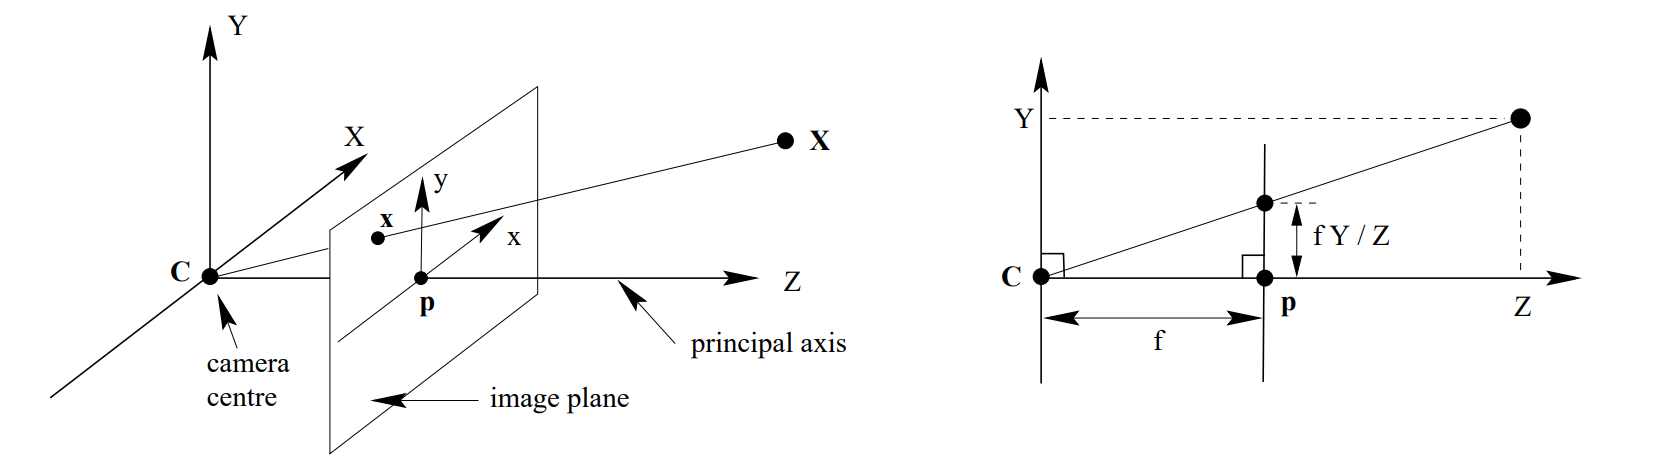
\includegraphics[width = \linewidth]{Images/pinholemodel.PNG}
    \caption{Pinhole camera model, taken from \cite{hartley2003multiple}}
    \label{fig:pinholemodel}
\end{figure}

Under the pinhole camera model, real-word points are projected onto the image plane (or focal plane) $Z = f$, resulting in a transformation from $\mathbb{R}^3$ to $\mathbb{R}^2$. More specifically, a point in space with coordinates $\vect{X} = (X,Y,Z)^T$ is mapped to the point where the line joining the point to the camera center, or center of projection, meets the image plane. The line perpendicular to the image plane passing for the camera center takes the name of principal axis, and its point of intersection with the image plane is the principal point. Using homogeneous coordinates, the pinhole camera model mapping is formalized in \cref{eq:pinholebase}.

\begin{equation}
\label{eq:pinholebase}
    \begin{pmatrix}
        fx\\
        fy\\
        z
    \end{pmatrix}=\begin{bmatrix}
    f_x & 0 & x_0 & 0 \\ 0 & f_y & y_0 & 0 \\ 0 & 0 & 1 & 0
    \end{bmatrix}\begin{pmatrix}
        X \\ Y \\ Z \\ 1
    \end{pmatrix} = \vect{K}\vect{X}
\end{equation}

In \cref{eq:pinholebase} $f_x$ and $f_x$ express the camera's focal length, i.e., the distance between the center of projection and the image plane. The variables $x_0$ and $y_0$ are the principal point offset, which are the principal point coordinates in the image reference frame, as presented in \cref{fig:pinhole2}. The focal length, principal point offset and camera's field of view are related by \cref{eq:fovfocal}.

\begin{equation}
\label{eq:fovfocal}
    f_x = \frac{x_0}{\mathrm{tan}(FOV_x / 2)}
\end{equation}

\cref{eq:pinholebase} can be rewritten in compact form as:

\begin{equation}
\label{eq:pinhole2}
    \vect{x} = \vect{K}\Upsilon_0 \vect{X}
\end{equation}

The matrix $\vect{K}$, explicitly defined in \cref{eq:pinholebase}, is the intrinsic camera matrix. The parameters of this matrix express the geometrical parameters of the camera. The term $\Upsilon_0$ expresses a rotation matrix that rotates the reference frame to have the y-axis pointing downward, as this is the convention commonly used for the image reference plane, as reported in \cref{fig:pinhole2}.
\begin{figure}[!ht]
    \centering
    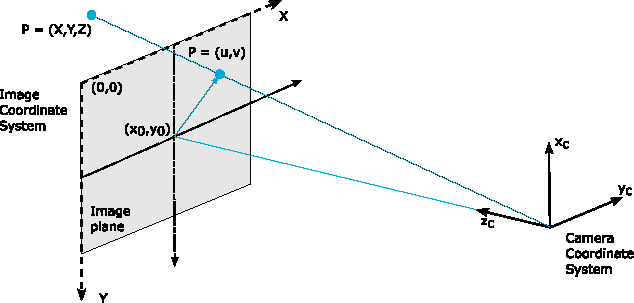
\includegraphics[width = 0.75\linewidth]{Images/pinhole1.pdf}
    \caption{Camera coordinate system and image coordinate system}
    \label{fig:pinhole2}
\end{figure}
\\The equations presented so far stand under the assumption that the position of the real-world point is known and expressed in the camera coordinate system. Commonly, the points to be projected by the camera model are expressed in a different coordinate system, generically called world reference frame. An example of this situation is reported in \cref{fig:pinhole3}. It is helpful to relate the mapping going from the position in the world reference frame to the image plane in a compact expression. \\

\begin{figure}[!ht]
    \centering
    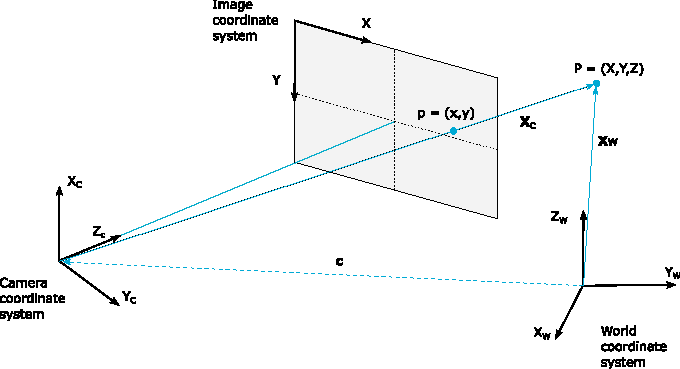
\includegraphics[width = 0.85\linewidth]{Images/pinhole2.pdf}
    \caption{Camera coordinate system and world coordinate system}
    \label{fig:pinhole3}
\end{figure}
By defining a three-element column vector $\vect{c}$ representing the camera center position in the world reference frame and a rotation matrix $\vect{R}$ that transforms the world coordinates into camera coordinates, the transformation between world coordinates to camera coordinates can be formalized as:
\begin{equation}
\label{eq:carttransform}
    \vect{X}^{cam} = \vect{R}\vect{X}^{world} - \vect{R}\vect{c}
\end{equation}
By defining the center of the world reference frame in camera coordinates as $\vect{t} = - \vect{R}\vect{c}$, and using homogeneous coordinates, \cref{eq:carttransform} can be rearranged as:
\begin{equation}
\label{eq:transfomogen}
    \vect{X}^{cam} = \begin{bmatrix}
        \vect{R} & \vect{t}\\ 0 & 1
    \end{bmatrix}\vect{X}^{world}
\end{equation}
Including \cref{eq:transfomogen} into \cref{eq:pinholebase} a mapping between a 3D point expressed in world coordinates and its position on the image plane is obtained:
\begin{equation}
    \vect{x}^{image} = \vect{K}\Upsilon_0 [\vect{R}|\vect{t}]\vect{X}^{world}
\end{equation}
It is therefore possible to define the projection matrix $\vect{P}$:
\begin{equation}
    \vect{P} = \vect{K}\Upsilon_0 [\vect{R}|\vect{t}]
\end{equation}
The projection matrix is the combination of the intrinsic parameters of the camera $\vect{K}$, representing its geometrical proprieties, and the extrinsic parameters $[\vect{R}|\vect{t}]$ that represent the camera position.


\subsection{2D Projective transformations}
\cref{fig:twoview} shows a scenario where a set of points with world coordinates $\vect{X}$ is observed from two cameras with projection centers $C_1$ and $C_2$, which have different poses. 
That condition can occur either in the case of two different cameras at different positions or where the same camera takes two consecutive images in time with relative camera-object motion. Those two camera histories mathematical description is anallogous \cite{hartley2003multiple}. 

\begin{figure}[!ht]
    \centering
    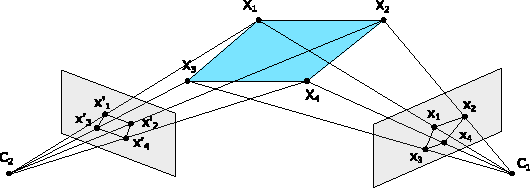
\includegraphics[width=0.9\linewidth]{Images/two-view.pdf}
    \caption{Same object multiple view}
    \label{fig:twoview}
\end{figure}

%The points' homogeneous coordinates on the image plane are respectively $\vect{x}$ and $\vect{x}'$.
$\vect{x}$ and $\vect{x}'$  represent the points homogenous coordinates on the image plane, respectively. 
The linear relationship between $\vect{x}$ and $\vect{x}'$ is named projective transformation, reported in \cref{eq:projective}.

\begin{equation}
\label{eq:projective}
    \vect{x}' = \vect{H}\vect{x} = \begin{bmatrix}
        h_1 &h_2 &h_3 \\ h_4 &h_5& h_6 \\ h_7 &h_8 &h_9
    \end{bmatrix}\vect{x}
\end{equation}

The matrix $\vect{H}$ is referred to as homography matrix. The transformation is defined by eight degrees of freedom, as the matrix is defined up to a scale \cite{dubrofsky2009homography}. This reflects the fact that the transformation relates homogeneous coordindates, which are also defined up to a scale. \\
Projective transformations can be seen as the generalization of simpler transformations, such as similarities and affine transformations. The detailed description of those transformations is beyond the thesis scope, the reader is referred to \cite{hartley2003multiple} for an in depth presentation of the subject.

%Further insight into those transformations is presented hereafter for the sake of completeness. 
% \subsubsection*{Similarity transformation}
% A similarity transformation (\cref{fig:similarity}) applies to the set of points a rotation, a translation, and isotropic scaling. The mathematical formalization of this transformation is given in \cref{eq:similariry}.

% \begin{equation}
%     \label{eq:similariry}
%     \vect{x}'= \vect{H}_S \vect{x} = \begin{bmatrix}
%         s\vect{R}(\vartheta) & \vect{t} \\ \vect{0}^T & 1
%     \end{bmatrix}\vect{x}
% \end{equation}

% In \cref{eq:similariry} $\vect{R}(\vartheta)$ is a $2 \times 2$ rotation matrix, $\vect{t}$ is a translation vector and $s$ the scaling factor. In the case $s$ is unitary, then the transformation takes the name of isometry.\\
% When a similarity transformation is applied, the angle between lines and the distance ratio between points don't change.

% \subsubsection*{Affine transformation}
% Affine transformations (\cref{fig:affine}) do not maintain the distance and angle between lines, but maintains the parallelism properties. \cref{eq:affine} is a generalisation of the similarity transformation.
% \begin{equation}
%     \label{eq:affine}
%     \vect{x}'= \vect{H}_A \vect{x} = \begin{bmatrix}
%         \vect{A} & \vect{t} \\ \vect{0}^T & 1
%     \end{bmatrix}\vect{x}
% \end{equation}

% where $\vect{A}$ is a  $2 \times 2$ non-singular matrix. $\vect{A}$ can be decomposed into the following concatenation of transformations:
% \begin{equation}
%     \vect{A} = \vect{R}(\vartheta) \vect{R}(-\phi)\begin{bmatrix}
%         \lambda_1 & 0 \\ 0 & \lambda_2
%     \end{bmatrix}\vect{R}(\phi)
% \end{equation}

% This set of transformations implies a first rotation of angle $\phi$, a scaling of entity $\lambda_1$ and $\lambda_2$ on the rotated $x$ and $y$ axis respectively, a rotation back of angle $\phi$, and a final rotation of angle $\vartheta$. Given this 4 degrees-of-freedom plus the two given by the translation $\vect{t}$, the affine transformation is defined by 6 degrees-of-freedom.

% \subsubsection*{Projective transformation}
% The transformations described so far do not necessarily require expressing points in homogeneous coordinates. This holds even in the case of affine transformations, as the last row of the matrix $\vect{H}$ equals $[0 \ 0 \ 1]$, so they can be considered as the concatenation of a non-singular linear transformation of Euclidean coordinates followed by a translation \cite{hartley2003multiple}.\\
% This is not the case with projective transformations (\cref{fig:projective}), the structure of which is given in \cref{eq:projectivestr}.
% \begin{equation}
%     \label{eq:projectivestr}
%     \vect{x}'= \vect{H}_P \vect{x} = \begin{bmatrix}
%         \vect{A} & \vect{t} \\ \vect{v}^T & v
%     \end{bmatrix}\vect{x}
% \end{equation}
% where $\vect{v} = [v_1 \ v_2]^T$. As only the ratio between the components of $\vect{H}$ is relevant, the transformation is defined by 8 degrees of freedom. 
% It is important to notice that for projective transformations, the mapping between the euclidean coordinates of the two sets of points is non-linear, unlike the transformations previously described.\\
% A projective transformation can always be decomposed into a chain of transformations:
% \begin{equation}
%     \label{Hdecompose}
%     \vect{H} = \vect{H}_S\vect{H}_A\vect{H}_P = \begin{bmatrix}
%         s\vect{R} & \vect{t} \\ \vect{0}^T & 1
%     \end{bmatrix}\begin{bmatrix}
%         \vect{J} &  \vect{0}\\\vect{0}^T & 1
%     \end{bmatrix}\begin{bmatrix}
%         \vect{I} &\vect{0} \\ \vect{v}^T& v
%     \end{bmatrix}
% \end{equation}
% where $I$ is the identity matrix and $J$ is an upper triangular matrix. Each transformation represents the essence of its type of transformation: $\vect{H}_S$ introduces the rotation translation and scaling, $\vect{H}_A$ affects the affine proprieties, and $\vect{H}_P$ introduces the projective deformation.\\
% A qualitative representation of the different types of transformations is given in \cref{fig:transformation}.
% \begin{figure}[!ht]
%      \centering
%      \begin{subfigure}[b]{0.3\textwidth}
%          \centering
%          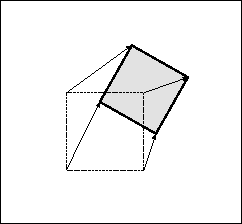
\includegraphics[width=\textwidth]{Images/rect5034.pdf}
%          \caption{Similarity transformation}
%          \label{fig:similarity}
%      \end{subfigure}
%      \hfill
%      \begin{subfigure}[b]{0.3\textwidth}
%          \centering
%          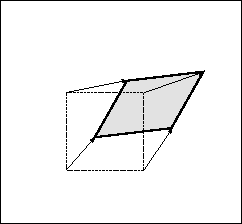
\includegraphics[width=\textwidth]{Images/rect5034-2.pdf}
%          \caption{Affine transformation}
%          \label{fig:affine}
%      \end{subfigure}
%      \hfill
%      \begin{subfigure}[b]{0.3\textwidth}
%          \centering
%          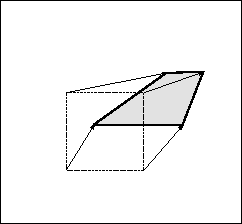
\includegraphics[width=\textwidth]{Images/rect5034-2-9.pdf}
%          \caption{Projective transformations}
%          \label{fig:projective}
%      \end{subfigure}
%         \caption{Examples of different transformations}
%         \label{fig:transformation}
% \end{figure}

\subsection{Direct Linear Transformation algorithm}
\label{toc:DLT}
Given a set of 2D to 2D point correspondences, estimating the homography between the two sets of points might be useful, as it encodes information about the relative pose of the two views \cite{hartley2003multiple}. Having the homography matrix 8 degrees of freedom, just four two-dimensional points are needed to estimate the transformation. A simple and effective algorithm to perform this is the Direct Linear Transformation (DLT) algorithm \cite{hartley2003multiple}. \\
If two points expressed in homogeneous coordinates $\vect{x}=[x \ y \ z]^T$ and $\vect{x}'=[x'\ y'\ w']^T$ satisfy the relation $\vect{x}'= \vect{H}\vect{x}$ (\cref{eq:projective}), than the following also must hold:
\begin{equation}
\label{eq:dim1eq1}
    \vect{x}' \times \vect{H}\vect{x} = \vect{0}
\end{equation}
%Denoting the $j$-th row of $\vect{H}$ by $\vect{h}^{T}_j$, it is possible to develop \cref{eq:dim1eq1} as:
The $j$-th row of $\vect{H}$ can be denoted as $\vect{h}^{T}_j$, so that \cref{eq:dim1eq1} becomes:
\begin{equation}
\label{eq:dim1eq2}
    \begin{pmatrix}
        y'\vect{h}^{T}_3\vect{x} - w'\vect{h}^{T}_2\vect{x}\\
        w'\vect{h}^{T}_1\vect{x} - x'\vect{h}^{T}_3\vect{x}\\
        x'\vect{h}^{T}_2\vect{x} - y'\vect{h}^{T}_1\vect{x}\\
        \end{pmatrix} = \vect{0}
\end{equation}

%Expressing \cref{eq:dim1eq2} as function of $[\vect{h}^{T}_1 \ \vect{h}^{T}_2 \ \vect{h}^{T}_3]^T$ it is possible to define a linear system with the components of the homography matrix as unknowns:
Equation \cref{eq:dim1eq2} can be expressed as function of $[\vect{h}^{T}_1 \ \vect{h}^{T}_2 \ \vect{h}^{T}_3]^T$ so to define a linear system with the components of the homography matrix as unknowns:
\begin{equation}
    \begin{bmatrix}
        \vect{0}^T & -w'\vect{x}^T  & y'\vect{x}^T\\
        w'\vect{x}^T & \vect{0}^T  & -x'\vect{x}^T\\
        -y'\vect{x}^T & x'\vect{x}^T &  \vect{0}^T\\
    \end{bmatrix}\begin{pmatrix}
        \vect{h}_1 \\ \vect{h}_2 \\ \vect{h}_3
    \end{pmatrix} =  \vect{0}
\end{equation}

Since two out of three are linearly independent equations, the system can be reduced to:

\begin{equation}
\label{eq:DLT}
    \begin{bmatrix}
        \vect{0}^T & -w'\vect{x}^T  & y'\vect{x}^T\\
        w'\vect{x}^T & \vect{0}^T  & -x'\vect{x}^T\\
    \end{bmatrix}\begin{pmatrix}
        \vect{h}_1 \\ \vect{h}_2 \\ \vect{h}_3
    \end{pmatrix} =  \vect{0}
\end{equation}

If the system in \cref{eq:DLT} is computed for four points it will result in a system with nine unknowns, namely the components of the homography matrix, and eight equations, thus resulting under-constrained. That highlights that only the ratio of the components of $\vect{H}$ is relevant. 
%By introducing a condition forcing the norm of the matrix to be unitary, a ninth equation is added to solve the under-constraining issue.\\
A condition to force the matrix norm to be unitary is introduced to solve the under-constraining issue.\\
If more than 4 point correspondences are considered, the system becomes over-determined; therefore, a least-square approach must be applied to find the solution. A practical way to solve the over-determined system is to apply the Singular Value Decomposition (SVD) to the matrix of coefficients and take the last vector of the matrix $\vect{V}$ as the solution.\\
%By defining the DLT algorithm as the solution of \cref{eq:DLT} a significant issue is overseen, i.e., the quality of the result is conditioned by the coordinate frame in which the points are expressed.
A significant issue is overseen whenever the DLT defines the \cref{eq:DLT} solution: the quality of the result is conditioned by the coordinate frame in which the points are expressed.
This implies that some reference frames provide better results than others. As suggested by \cite{hartley2003multiple}, a normalization to the points sets to increase the DLT algorithm's performances can be applied. The normalization consists of defining two transformations $\vect{T}$ and $\vect{T}'$ respectively for the sets of points $\vect{x}$ and $\vect{x}'$ that translate the centroid of the sets at the origin and scales them such than their average distance from the origin equals $\sqrt{2}$. Once this normalization is applied, \cref{eq:DLT} cab be solved and then the matrix  $\vect{H}$ denormalized. The complete DLT algorithm is summarised in \cref{alg:DLT}.

\begin{algorithm}
\caption{Normalized DLT for 2D homographies \cite{hartley2003multiple}}\label{alg:DLT}
\begin{algorithmic}[1]
\State Given at least 4 2D to 2D point correspondences $\vect{x}\rightarrow\vect{x}'$ 

\State Compute the normalization of $\vect{x}$ such that $\tilde{\vect{x}} = \vect{T}\vect{x}$ 
\State  Compute the normalization of $\vect{x}'$ such that $\tilde{\vect{x}}' = \vect{T}'\vect{x}'$ 
\State Solve the linear system in \cref{eq:DLT} using the normalized coordinates to obtain the homography $\tilde{\vect{H}}$
\State  Denromalize the homography matrix such that $\vect{H} = \vect{T}'\tilde{\vect{H}}\vect{T}$
\end{algorithmic}

\end{algorithm}

\subsection{Random Sample Consensus method}
\label{sec:RANSAC}
The DLT algorithm, presented in Section \ref{toc:DLT}, assumes that the position of points on the image plane is not affected by noise and that outliers (elements following a different, and possibly unmodelled,
error distribution \cite{hartley2003multiple}) don't exist in the set considered. A widespread algorithm for model fitting data containing spurious points is the RANSAC method, introduced by Fischler and Bolles in \cite{fischler1981random}.\\
The RANSAC algorithm, summarised in \cref{alg:RANSAC}, starts by randomly selecting the minimum number of correspondences required for the model fitting (4 for the homography), and computes the model based on the values selected. It then uses the newly fitted model to compute the number of inliers, evaluating the distance of the points from the fitted model. This process is repeated iteratively until the exit condition is reached. The algorithm's output is the model that maximizes the number of inliers. 
\begin{algorithm}
\caption{RANdom SAmple Consensus (RANSAC) \cite{fischler1981random}}\label{alg:RANSAC}
\begin{algorithmic}[1]
\State Let $A$ be a set of $N$ correspondaces
\While{$n_{iter} < n_{max}$ and $\epsilon > \epsilon_{max}$}
\State Select a sample $s$ from the set $A$
\State Fit the model to $s$
\State Compute the distance of all points in $A$ from this model
\State Compute the inliers set and the percentage of outliers $\epsilon_i$
\If{$\epsilon_i<\epsilon$}
\State Update $\epsilon$ and save model
\EndIf
\EndWhile
\end{algorithmic}
\end{algorithm}

RANSAC is an iterative and non-deterministic algorithm. This implies that the result is not repeatable. It depends on the randomness of the selected points to fit the model, and its accuracy depends on the maximum number of iterations. Therefore, the number of iterations is selected high enough to ensure with a given probability $p$ that at least one of the selected random sets does not include any outliers. The maximum number of iterations $n_{max}$ can be computed as:
\begin{equation}
    n_{max} = \frac{log(1-p)}{log(1-(1-\epsilon)^s)}
\end{equation}
\cref{fig:ransac} reports an example of RANSAC applied to the case of a line-fitting problem. It can be observed that the least squares fit is highly influenced by the presence of the outliers, while the RANSAC fit is more consistent with the inliers.
However, it is possible to obtain an even more reliable solution to the problem by adding a step to the RANSAC algorithm. Once the RANSAC model and the inliers set are computed, applying the least squares fit to all the correspondences in the inliers set provides the best estimate of the model, as seen in \cref{fig:ransac}. In the case of homography estimation, this procedure takes the name of Gold Standard Algorithm \cite{hartley2003multiple}, as it provides the best estimate of the homography matrix. 

\begin{figure}[!ht]
    \centering
    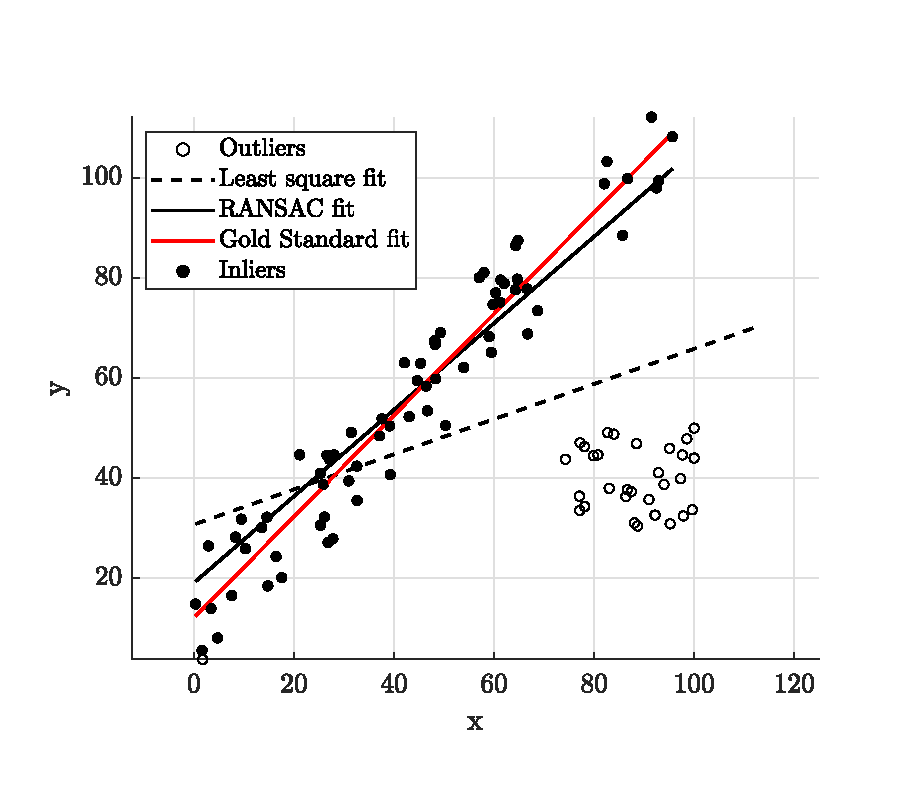
\includegraphics[clip,trim= 0cm 0.5cm 0cm 0cm,width = 0.7\linewidth]{Images/ransac.eps}
    \caption{Example of line fitting with different algorithms}
    \label{fig:ransac}
\end{figure}


\subsection{Point features}
\chaptermark{Background}
\label{sec:features}
In Computer Vision, a feature is generally defined as a distinguishable element of an image. Features can be of many types, such as points, edges, circles, or colors \cite{rondao2020benchmarking}. The following sections further detail the concept of point features, also known as keypoints or corner features, introducing the most common methods to detect describe and track these features. 
%The thesis exploits the point features, also referred to as keypoints or corner features; thus, the following sections will introduce the most common methods to detect, describe and track these features.

\subsubsection*{Features detection \& extraction}
Feature detection is a process that aims to identify for each image point if it corresponds to a feature. The output is a set of points coordinates, subset of the image pixels position, corresponding to each feature identified. Methods for point features detection can be divided into two categories: 
\begin{itemize}
    \item \textit{corner detectors}, which identifies the intersection between two edges;
    \item  \textit{blob detectors}, which detect features by considering a supporting surrounding region.
\end{itemize}
Once the features location is identified, a neighboring region can be defined and encoded into a numerical descriptor. That process refers to as \textit{feature extraction} or \textit{feature description}, and it enables matching the same feature in different images without searching the whole image.\\
Different point features detectors and descriptor can be found in literature. A detailed overview of the most common and an evaluation of their applicability for multispectral navigation is reported in \cite{rondao2020benchmarking}, highlighting a better performance of blob detectors for thermal images. Although modeled equally from a geometrical perspective, visible and thermal images present an overall difference in appearance, requiring different considerations in terms of features detection. \\
The selection process of the methods used in the thesis is based on a trade-off between edge detectors methods and blob detectors reported in \cref{tab:dectmeth}. That set of algorithms includes both methods for detection only and both detection and extraction because, as explained in in the Feature tracking paragraph of \cref{toc:fftrack}, the feature descriptors are not adopted in this work.\\
\begin{table}[!h]
    \centering
    \begin{tabular}{p{2cm} p{3.5cm} p{5cm} l}
        Method & Type & Function & Reference \\\hline \hline
        FAST & Corner detector & Detection & \cite{rosten2005fusing} \\\hline
        ORB & Corner detector & Detection \& description & \cite{rublee2011orb}\\\hline
        BRISK & Corner detector & Detection \& description & \cite{leutenegger2011brisk}\\\hline
        SIFT & Blob detector & Detection \& description & \cite{lowe2004sift}\\\hline
        SURF & Blob detector & Detection \& description & \cite{bay2006surf}\\ \hline
         
    \end{tabular}
    \caption{Features detection methods evaluated in the thesis work}
    \label{tab:dectmeth}
\end{table}

The detailed description of these methods is outside the scope of this work, which focuses on their application. For a detailed description of the algorithms the reader is referred to their formulation in the related papers \cite{rosten2005fusing,rublee2011orb,leutenegger2011brisk,lowe2004sift,bay2006surf}.\\
% \begin{figure}[!ht]
%      \centering
%      \begin{subfigure}[b]{0.45\textwidth}
%          \centering
%          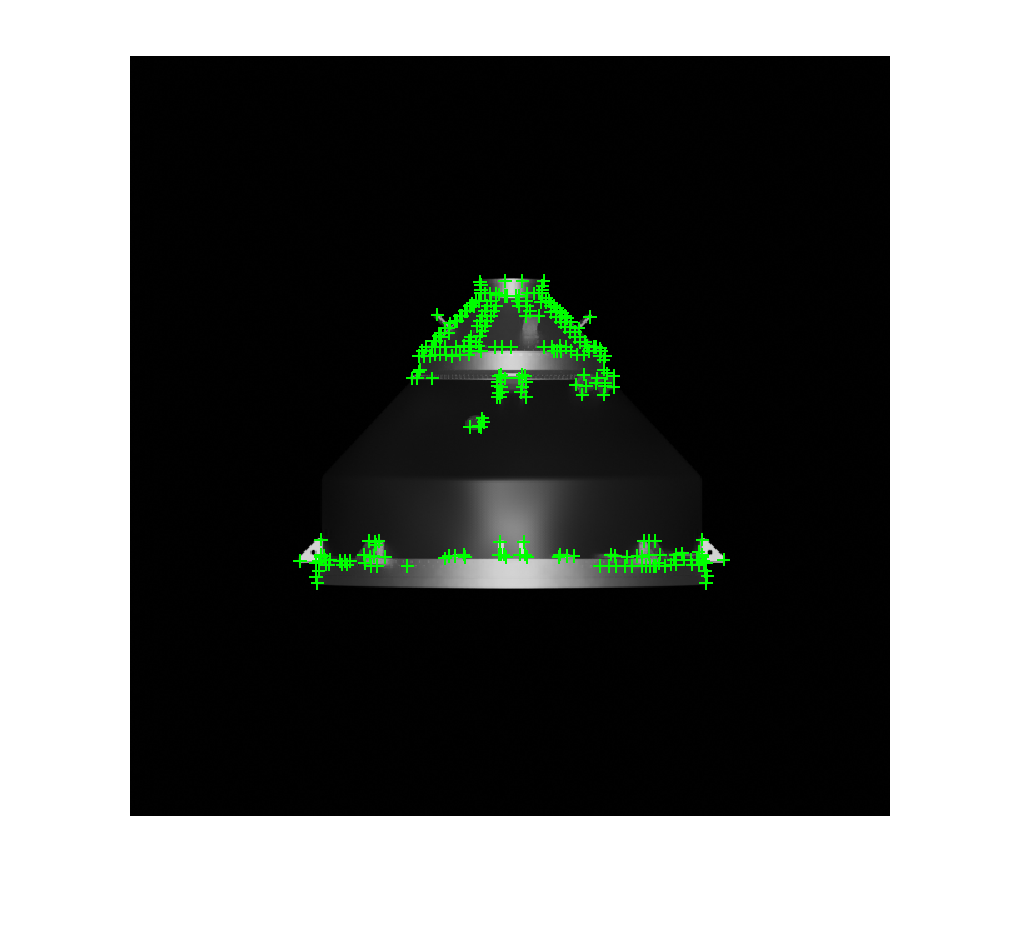
\includegraphics[clip,trim = 1cm 0cm 1cm 0cm,width=\textwidth]{Images/orb.eps}
%          \caption{ORB features on a visible image}
%          \label{fig:orb}
%      \end{subfigure}
%      \hfill
%      \begin{subfigure}[b]{0.45\textwidth}
%          \centering
%          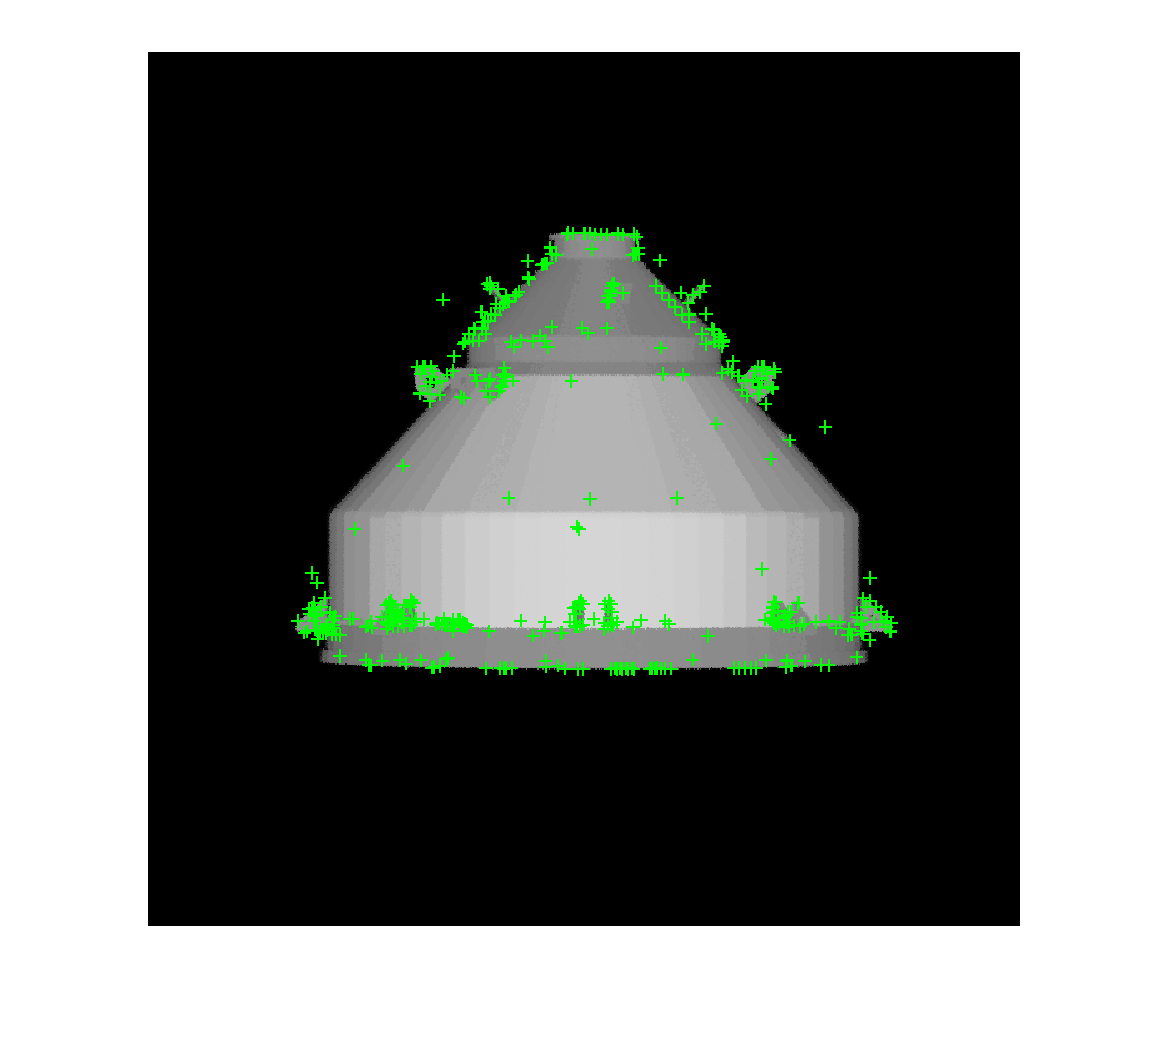
\includegraphics[clip,trim = 1.15cm 0cm 1.15cm 0cm,width=\textwidth]{Images/sift.eps}
%          \caption{SIFT features on a thermal image}
%          \label{fig:surf}
%      \end{subfigure}
%         \caption{Examples of different feature detection methods}
%         \label{fig:detection}
% \end{figure}
As the feature detection process is highly dependent on the pixel intensity in the image \cite{rondao2020benchmarking}, whenever a scarce contrast within the image holds the number of detected features is limited. That typically happens while processing thermal images whenever the temperature profile is almost uniform within the target and visible images whenever the target is in shadow. 
%A solution to this issue is to pre-process the image before the features detection applying an histogram equalization. 
The image pre-processing beforehand the feature extraction through histogram equalization mitigates those issues.
This process consists into splitting the image into different tiles, and then equalizing the pixel intensity so to increase the contrast and enhance the edges. In particular, the Contrast Limited Adaptive Histogram Equalization (CLAHE) \cite{zuiderveld1994contrast} algorithm successfully avoids overshooting in the contrast in sections with a uniform texture, like the background of the image. An example on the effect of CLAHE on a thermal image can be appreciated comparing \cref{fig:CLAHEbefroe} and \cref{fig:CLAHEafter}.

\begin{figure}[!h]
\captionsetup[subfigure]{labelformat=empty}
\begin{subfigure}[a]{0.42\linewidth}
\centering
    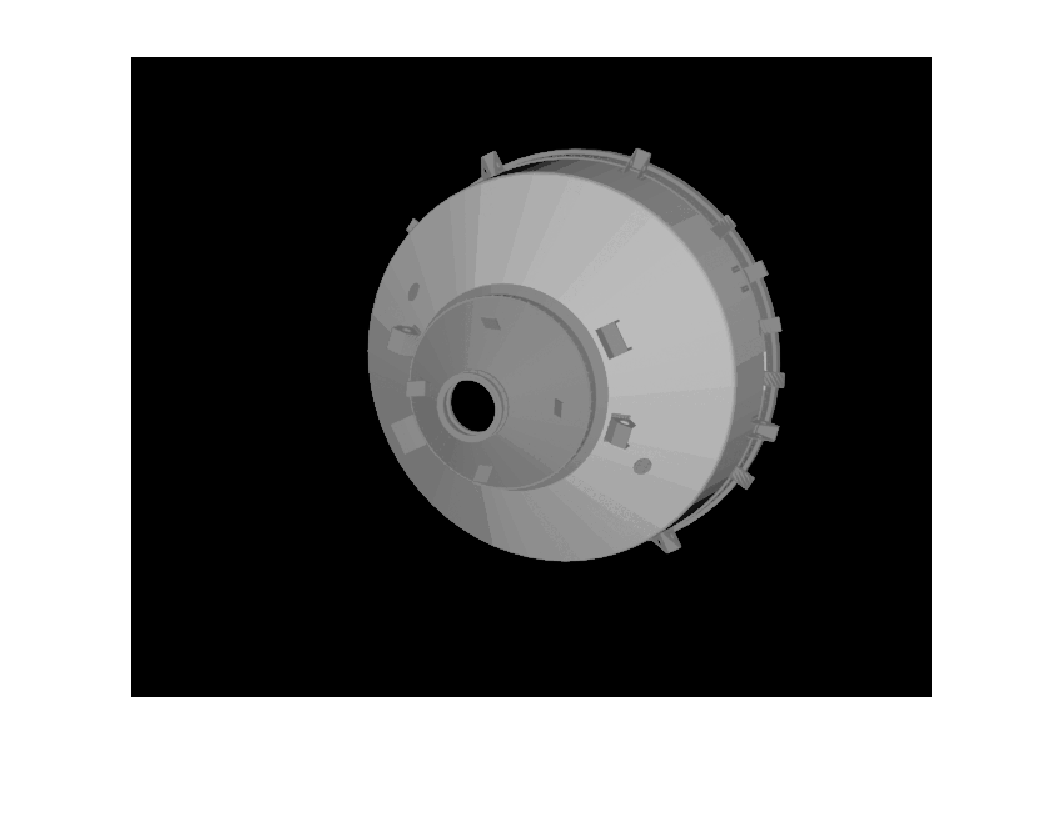
\includegraphics[width=\linewidth]{Images/imgCLAHEbefore.eps}
\end{subfigure}\hfill
\begin{subfigure}[a]{0.55\linewidth}
\centering
    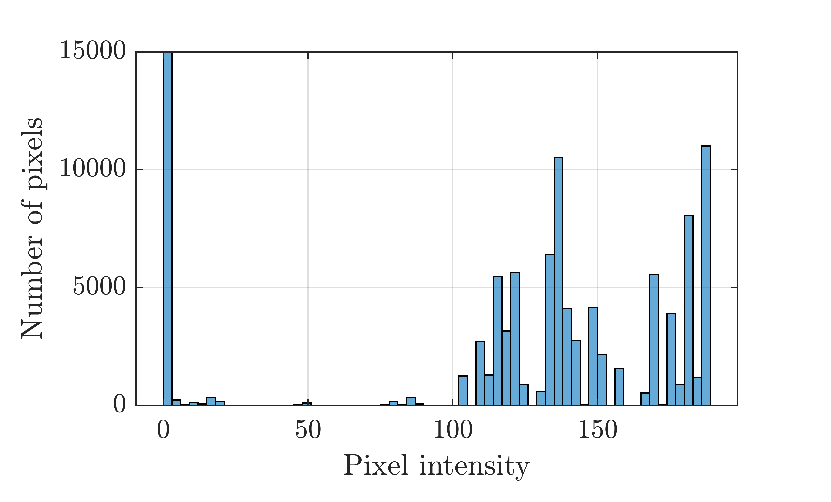
\includegraphics[width=\linewidth]{Images/CLAHEbefore.eps}
\end{subfigure}
    \caption{Thermal image and intensity histogram before applying CLAHE}
    \label{fig:CLAHEbefroe}
\end{figure}
\begin{figure}[!h]
\captionsetup[subfigure]{labelformat=empty}
\begin{subfigure}[a]{0.42\linewidth}
\centering
    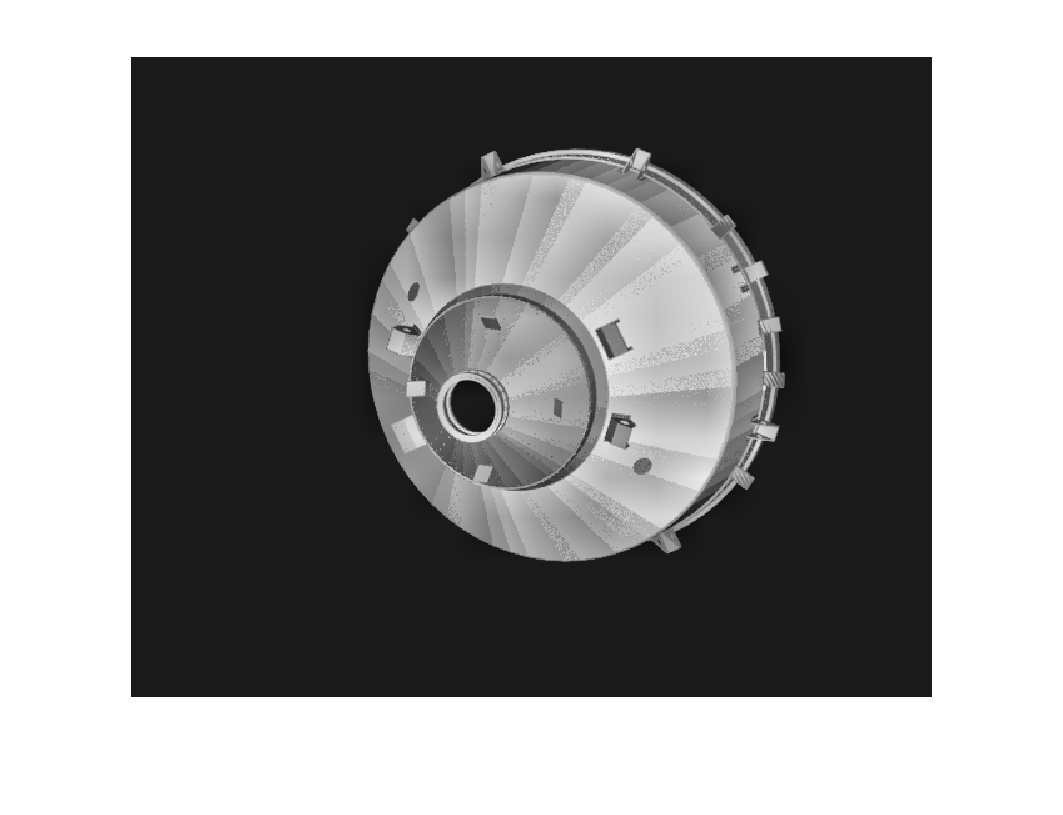
\includegraphics[width=\linewidth]{Images/imgCLAHEafter.eps}
\end{subfigure}\hfill
\begin{subfigure}[a]{0.55\linewidth}
\centering
    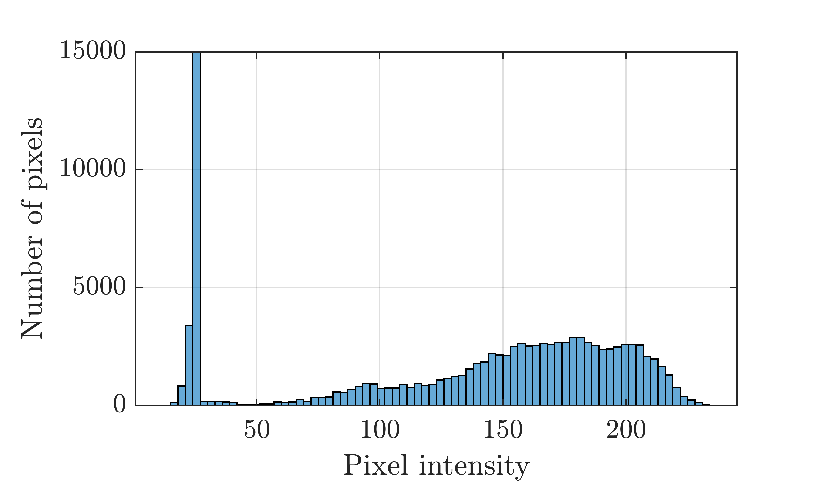
\includegraphics[width=\linewidth]{Images/CLAHEafter.eps}
\end{subfigure}
    \caption{Thermal image and intensity histogram after applying CLAHE}
    \label{fig:CLAHEafter}
\end{figure}

\subsubsection*{Features tracking}
\label{toc:fftrack}
%For visual navigation, it is useful to find the location of the same features on subsequent images taken from a different pose once a set of features is extracted from an image. 
Visual navigation benefits from tracking same features in subsequent images. 
This problem is commonly referred to as \textit{feature tracking}. A straightforward solution would be for each image to extract a new set of features, then match them with the original set using the descriptor information. However, this solution might result in a heavy computational burden, making it less suitable for onboard execution. In optical navigation applications, if the frame rate of acquisition of the images is in the order of seconds, the pose difference between two consecutive images is limited. This enables to use \textit{feature tracking} techniques that extract keypoints only in the first image and track them in consecutive images searching for them in a bounded spot around the previous position.
%to extract key points from the first image only to track them in the consecutive image, searching for them in a bounded region around the previous one. 
The output of each step is the field of displacement of the features between two consecutive images, known as \textit{optical flow}.\\
%When using feature tracking algorithms, 
Whenever feature tracking algorithms are adopted, 
two aspects have to be considered. Firstly, some features might be erroneously tracked, asking for an outlier rejection routine such as RANSAC at each step to remove spurious results. Secondly, the number of features will strictly decrease over time: that happens as the features are detected in the first image only, and over time they might either move outside the camera's field of view or get shadowed, as can be seen in \cref{fig:track}. To tackle those issues, the detection step shall be revisited as soon as the number of tracked key points gets below a defined threshold.\\
A widely used algorithm to perform feature tracking is the Lucas-Kanade (LK) tracker \cite{lucas1981iterative}. This algorithm associates a movement vector to every key point from its position in the first image to the position in the second image. To register the position of the key points in the two images, three assumptions hold:
\begin{itemize}
    \item the color of a pixel, or its intensity in gray scale images, does not change over two consecutive images. 
    \item The motion of the keypoints is limited to a bounded neighboring region around its original position.
    \item The keypoints are assumed to lie on rigid objects, thus moving coherently.
\end{itemize}
 The research adopts the pyramidal version of the LK algorithm implemented in the MATLAB computer vision toolbox. As a detailed description of the algorithm is outside the scope of this work, which focuses on its application, the reader is referred to \cite{baker2004lucas} and \cite{bouguet2001pyramidal} for an overview of the different LK formulations and the implementation of the pyramidal LK respectively.\\
\begin{figure}[!ht]
     \centering
     \begin{subfigure}[b]{0.32\textwidth}
         \centering
         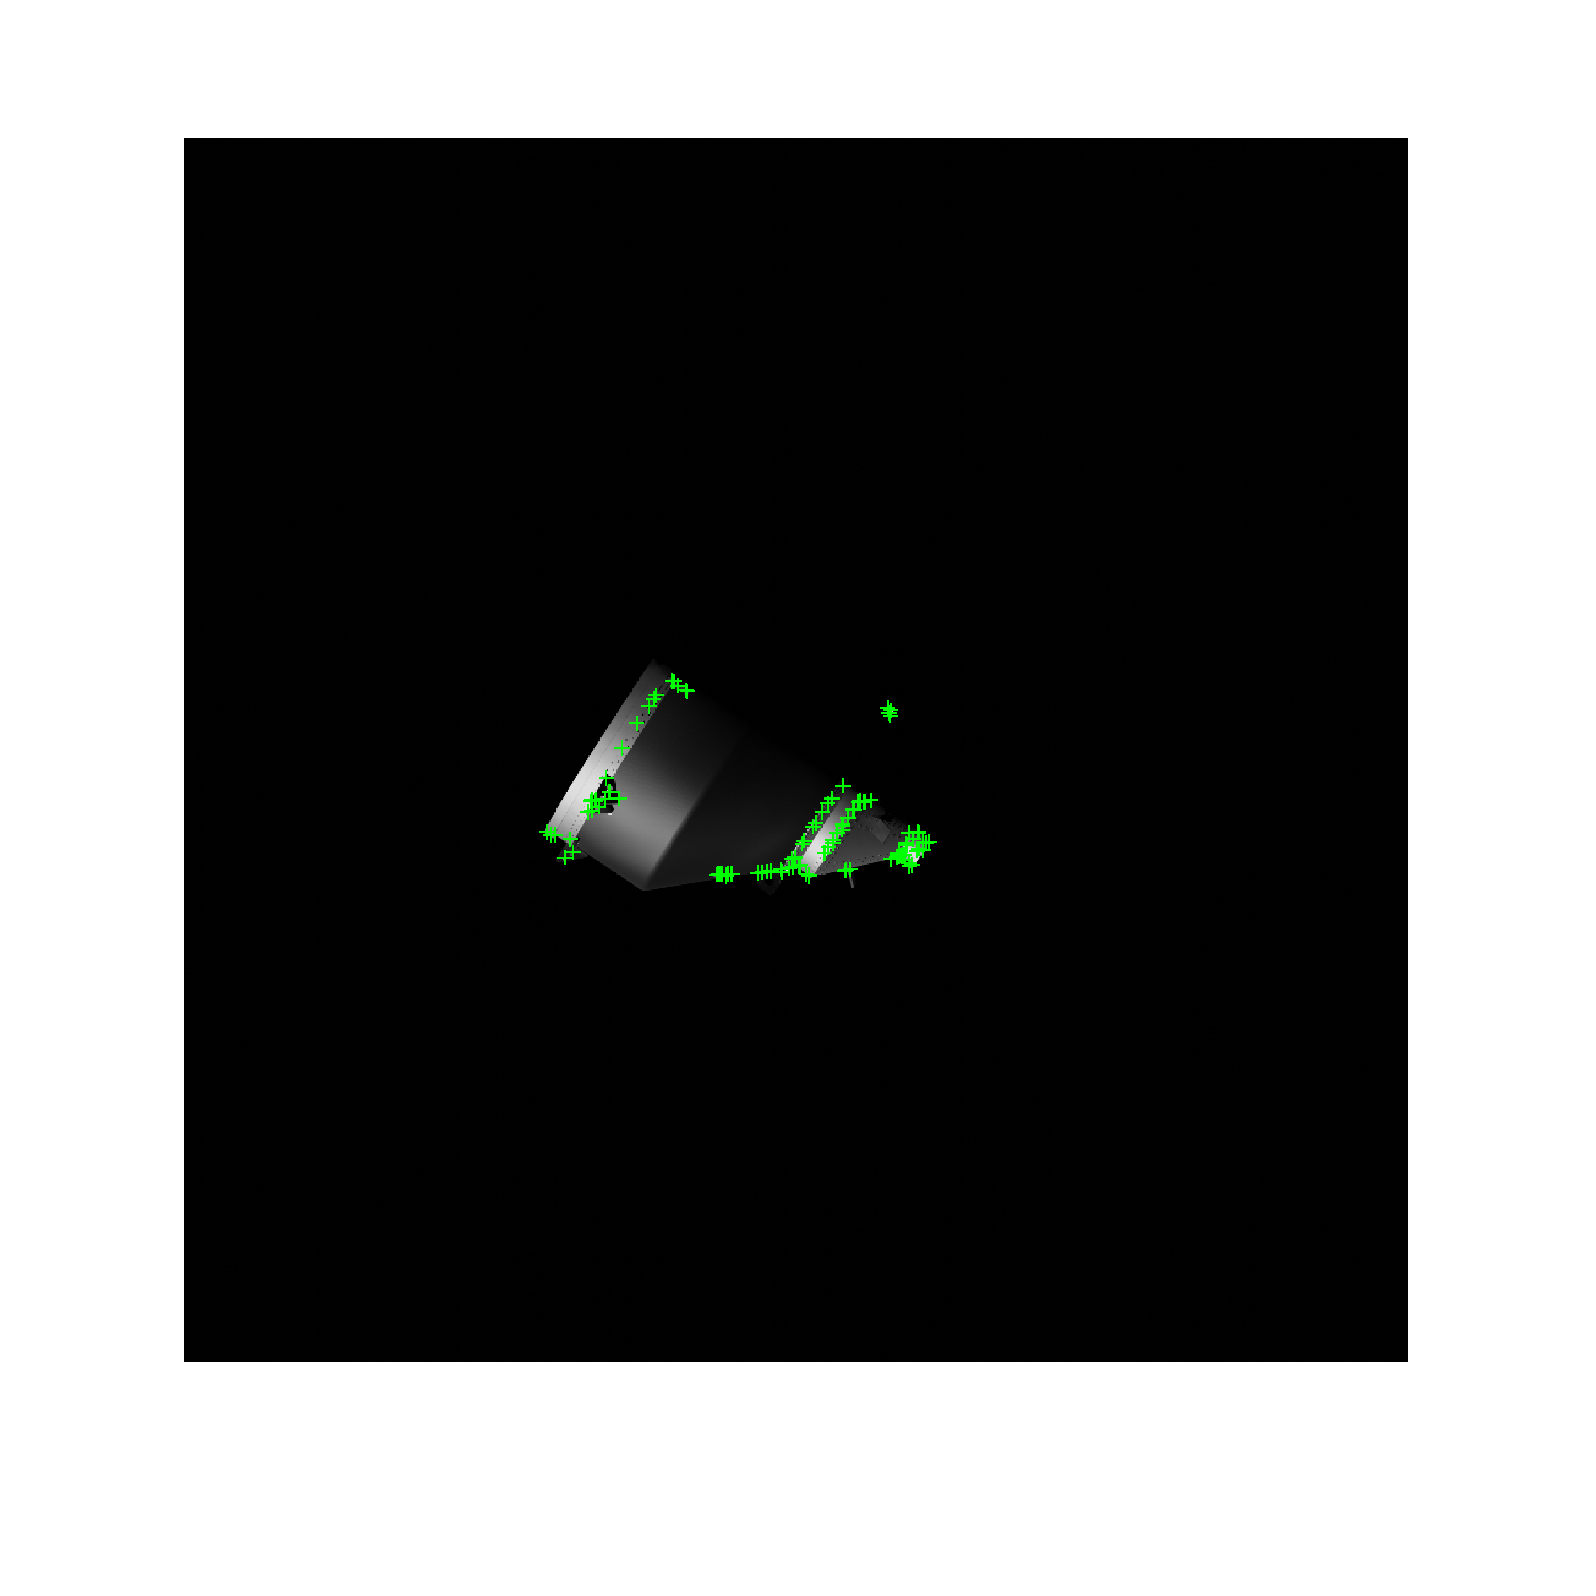
\includegraphics[clip,trim= 6cm 6cm 6cm 6cm,width=\textwidth]{Images/t0.eps}
         \caption{Detected keypoints \quad \mbox{} \quad \quad (n. = 115)}
         \label{fig:t0}
     \end{subfigure}
     \hfill
     \begin{subfigure}[b]{0.32\textwidth}
         \centering
         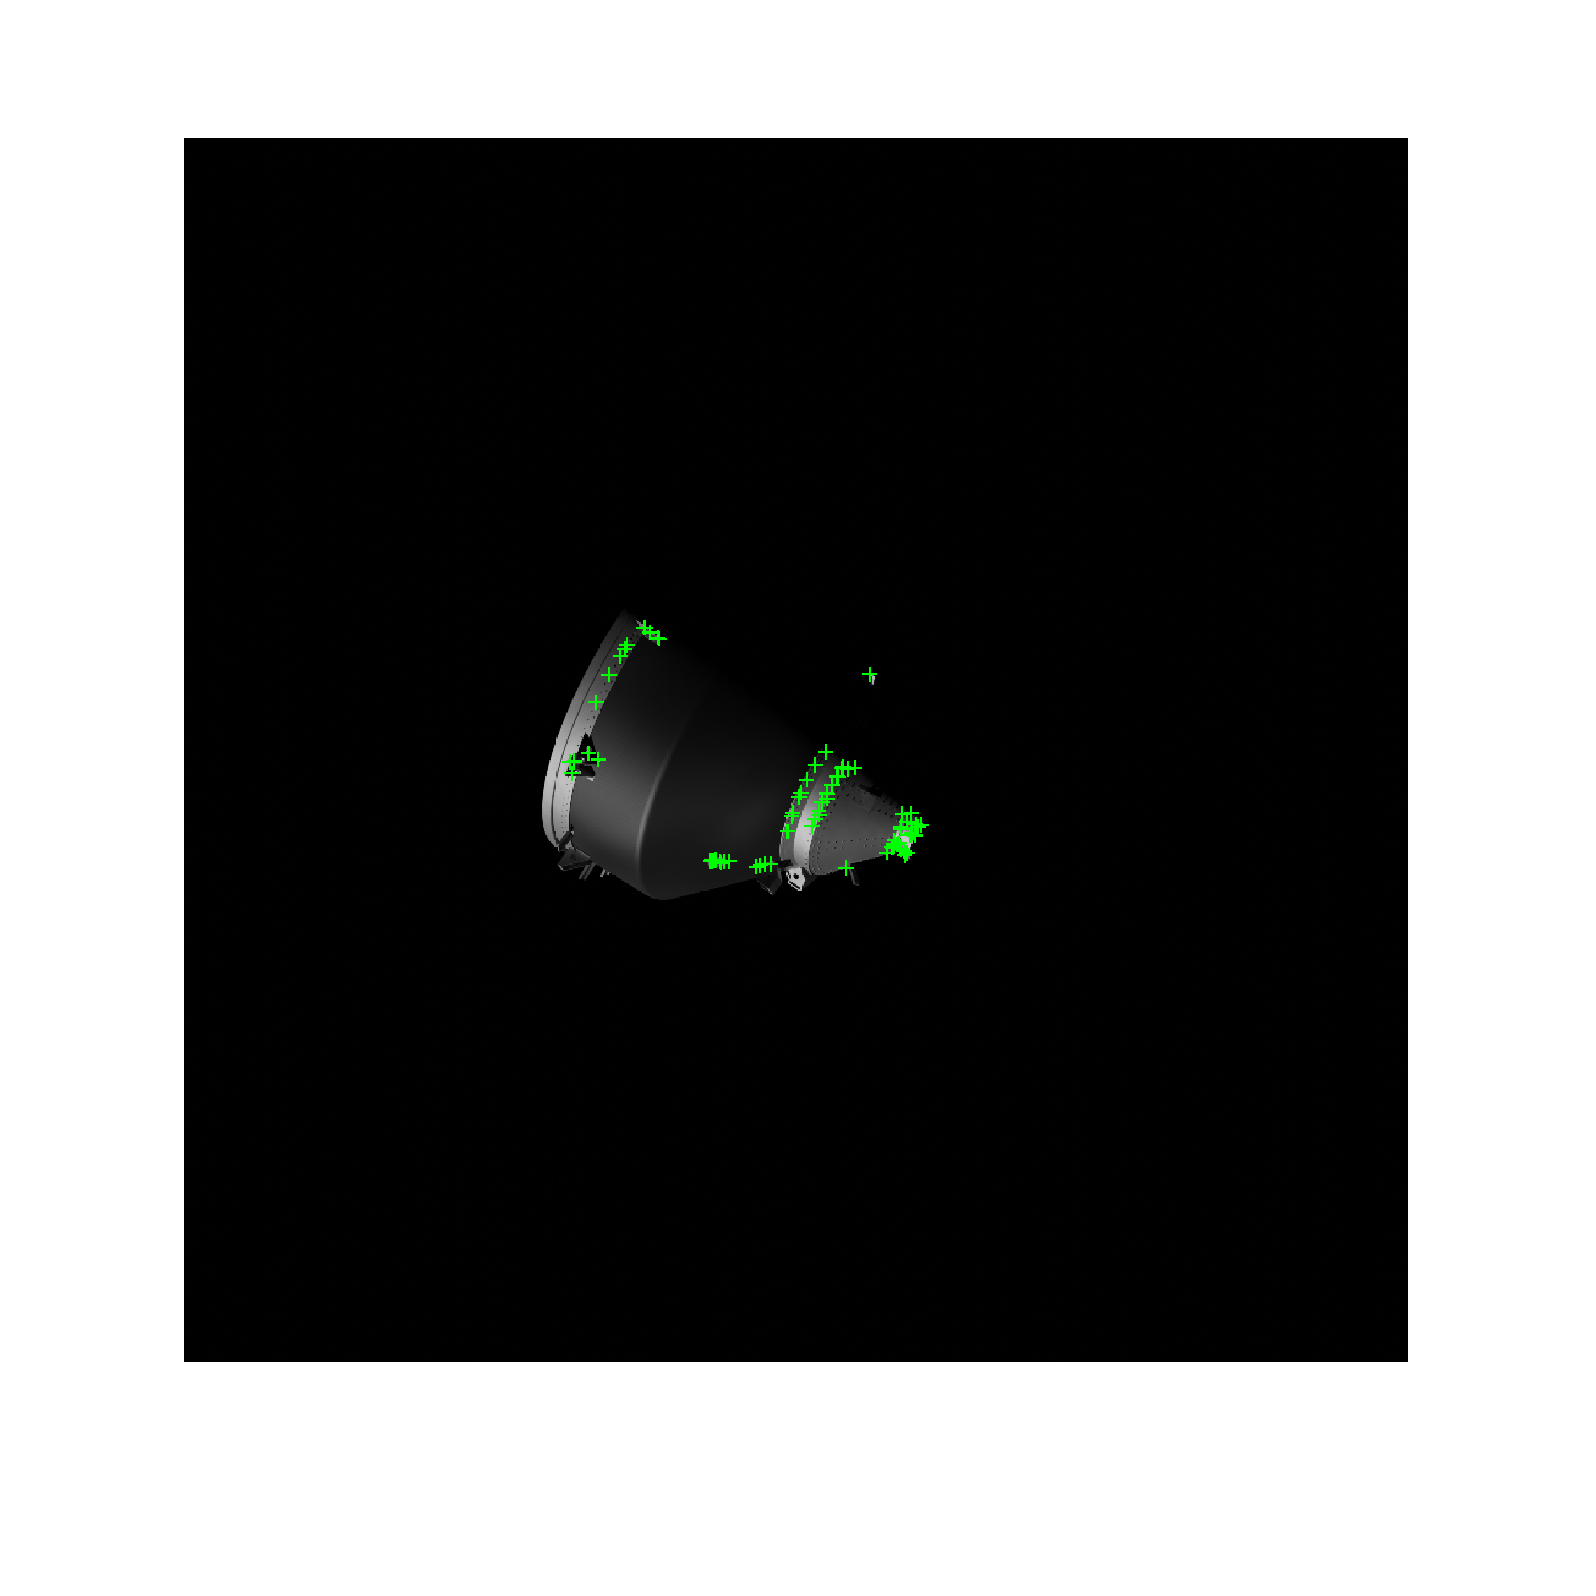
\includegraphics[clip,trim= 6cm 6cm 6cm 6cm,width=\textwidth]{Images/t30.eps}
         \caption{Tracked keypoints (n. = 85) after $\SI{30}{\second}$}
         \label{fig:t30}
     \end{subfigure}
     \hfill
     \begin{subfigure}[b]{0.32\textwidth}
         \centering
         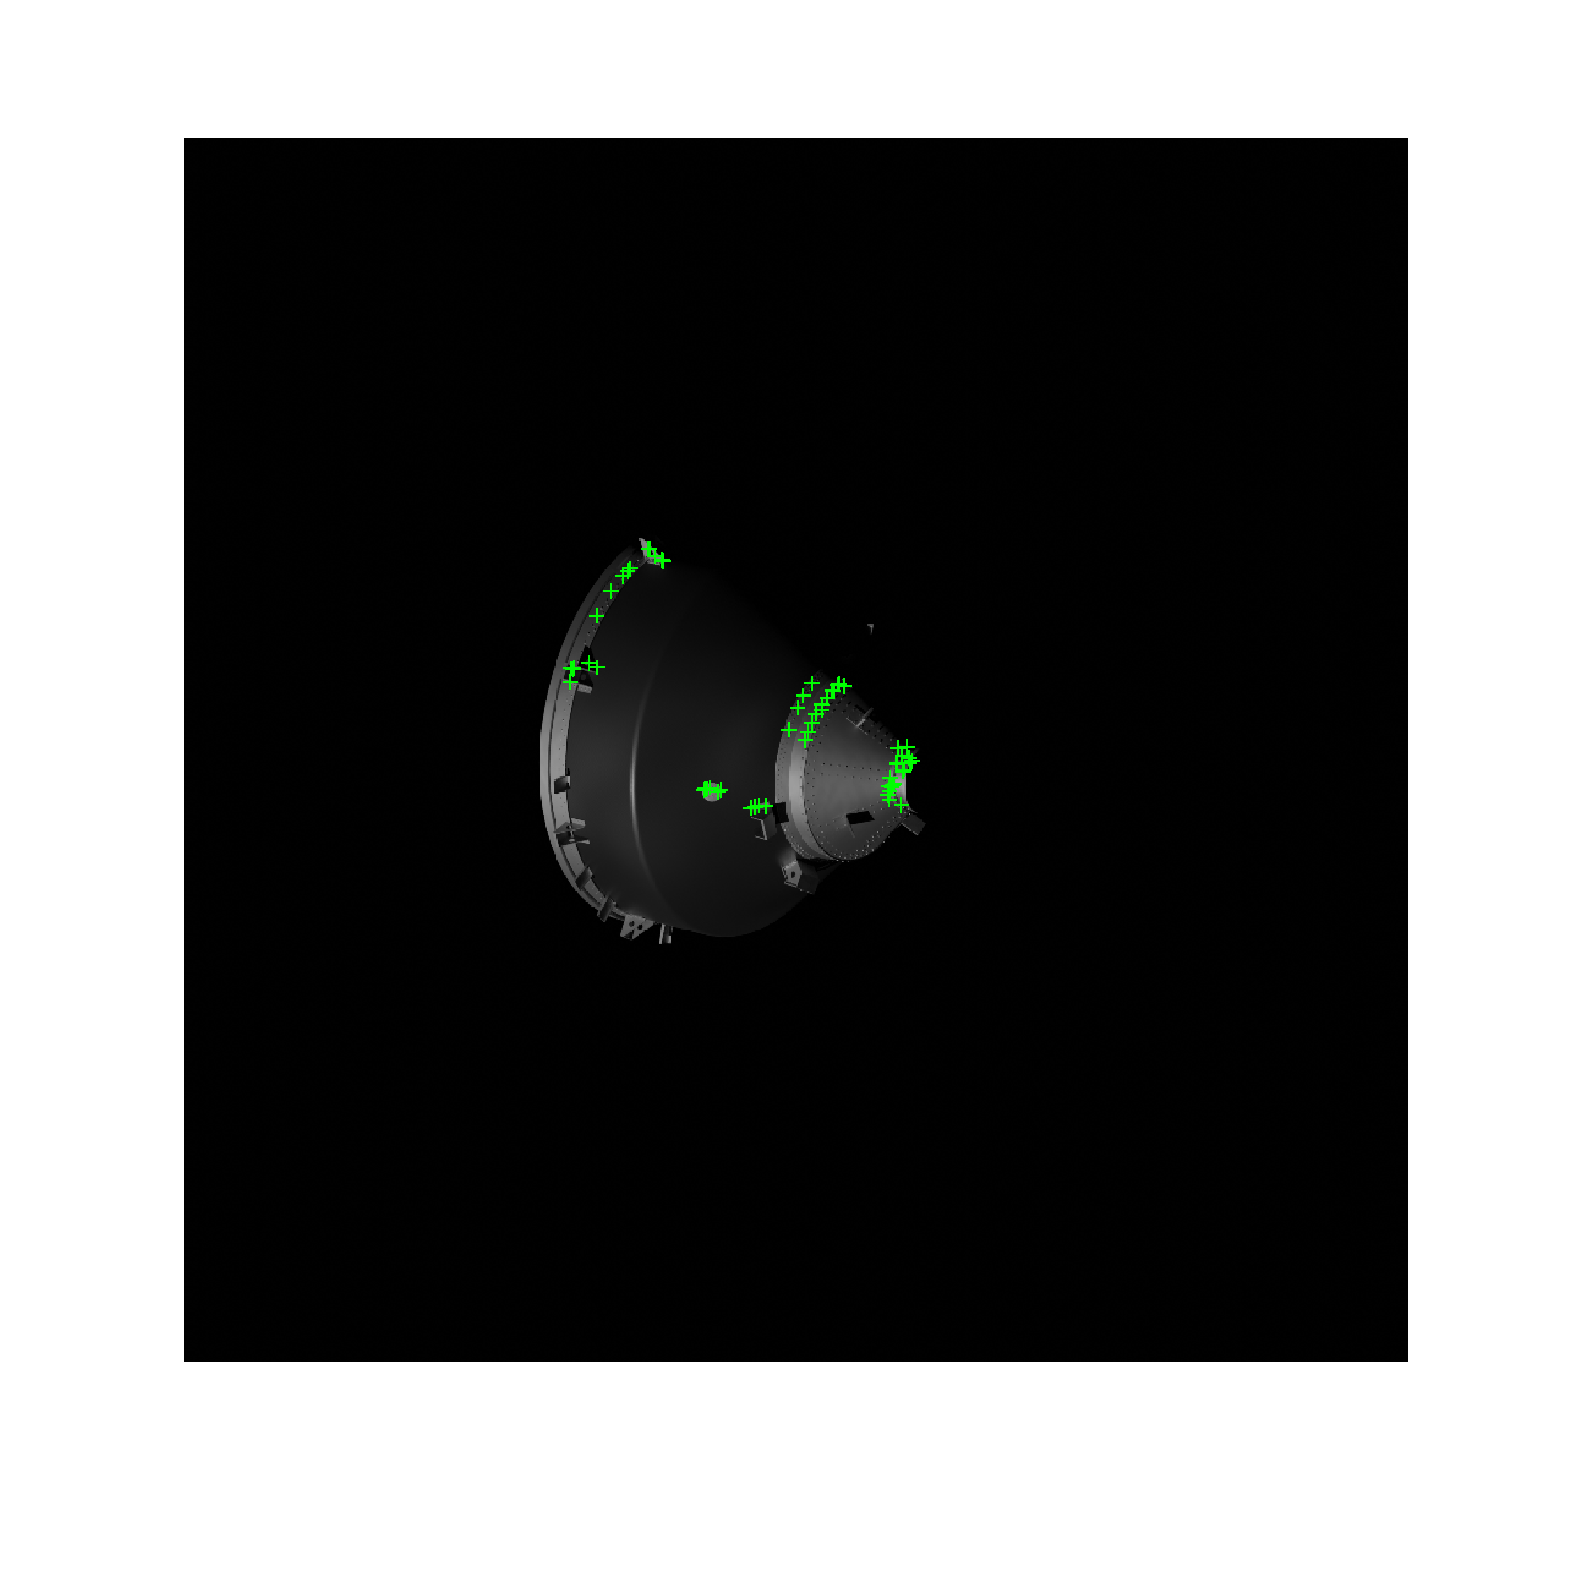
\includegraphics[clip,trim= 6cm 6cm 6cm 6cm,width=\textwidth]{Images/t60.eps}
         \caption{Tracked keypoints (n. = 67) after $\SI{60}{\second}$}
         \label{fig:t60}
     \end{subfigure}
        \caption[Features tracked with the LK algorithm]{Features tracked with the LK algorithm in different frames taken at a frequency of $\SI{1}{\hertz}$ with a relative angular rate of $\SI{1.5}{\deg\per\second}$}
        \label{fig:track}
\end{figure}


\section{Non-linear estimation}\chaptermark{Background}
In vision-based navigation, the features tracked on the image represent the primary source of information from the sensors. However, feature detection and tracking are always subject to a certain degree of noise, propagating into the pose information. Moreover, the information given by the position of the features at a given time is not directly influenced by the relative velocity or the angular rates, thus making their direct determination impossible without considering a sequence of measurements. This is commonly referred to as the observability problem of dynamical systems. \\
%Because of its broad implementation and straightforward formulation, a filter-based approach based on the Kalman Filter was selected for this work. 
For the thesis work a filtering approach based on the Klaman Filter (KF) was selected because its capability to deal with nonlinear dynamics and measurements functions while maintaining a lightweight implementation. 
The Kalman Filter is a first-order Bayesian filter that iteratively predicts the states' estimates propagating them with a dynamical model (prediction step) to update the prediction with the information from the measurements (correction step). In the interest of brevity, the demonstration and formulation of the Kalman filter are not reported. For a detailed explanation of the method, the reader is referred to \cite{zarchan2005progress}.\\
The classic formulation of the Kalman Filter works for linear systems only, while the relative navigation problem is intrinsically non-linear \cite{pesce2019comparison}. The filter's formulation has been extended to deal with non-linearity with the Extended Kalman Filter (EKF) and the Unscented Kalman Filter (UKF). The latter is less computationally efficient but is more accurate than the EKF, as it does not require any linearization of the dynamics.
Because the thesis applies to close-proximity operations with short measurement update intervals, making the nonlinearity less problematic, the EKF was considered the most effective solution. 
%Because the navigation applications require a high-frequency measurement update, making the non-linearity less problematic, the EKF was considered the most effective solution for these applications.

\subsection{The Extended Kalman Filter}
To introduce the EKF, it is first necessary to describe the real world set of non-linear differential equations describing the system:
\begin{align}
    \label{eq:EKF1}
    \dot{\vect{x}} & = f(\vect{x}) + \boldsymbol{w}\\
    \label{eq:EKF2}
    \vect{y} & = h(\vect{x}) + \boldsymbol{v}
\end{align}
where $\vect{x}$ is the vector of system states, $\vect{y}$ is the vector of measurements, $f(\vect{x})$ is the nonlinear function of the states and $h(\vect{x})$ is the measurement function that maps the states into the measurements. $\boldsymbol{w}$ and $\boldsymbol{v}$ are zero mean gaussian noises with known covariance such that:
\begin{align}
    \label{eq:COV1}
    \vect{Q}& = E(\boldsymbol{w}\boldsymbol{w}^T)\\
    \label{eq:COV2}
    \vect{R}& = E(\boldsymbol{v}\boldsymbol{v}^T)
\end{align}
where $E(\,\cdot\,)$ denotes the expected value. $\vect{Q}$ and $\vect{R}$ are referred to as process noise matrix and measurement noise matrix respectively. \\
To make the classical Kalman Filter formulation applicable to non-linear problems, in the EKF the both the state and the measurement functions are linearized in the current state estimate, computing the Jacobian matrices of the two functions:
\begin{align}
\label{eq:DER1}
    \vect{F}& = \dfrac{\partial f(\vect{x})}{\partial \vect{x}}\Big\vert_{\vect{x} = \hat{\vect{x}}}\\[1ex]\label{eq:DER2}
    \vect{H}& = \dfrac{\partial h(\vect{x})}{\partial \vect{x}}\Big\vert_{\vect{x} = \hat{\vect{x}}}
\end{align}
Further, to propagate the covariance matrix between two consecutive time steps, it is necessary to compute the state transition matrix $\Phi$. This can be performed with a variety of approaches, such as finite differences, variational approach or exponential matrix. 
% However, in most application a second order truncation of the Taylor series expansion (\cref{eq:taylor}) is sufficient \cite{zarchan2005progress}.
% \begin{equation}
% \label{eq:taylor}
%     \Phi(t,t_0) = \vect{I} + \vect{F}\Delta t + \vect{F}^2 \dfrac{\Delta t^2}{2}+ \vect{F}^3 \dfrac{\Delta t^3}{3!}+...
% \end{equation}
With this linearization it is possible to consider the system to be linear at each step of the filter. The steps of the Extended Kalman Filter are reported in \cref{alg:EKF}.

\begin{algorithm}[!ht]
\caption{Extended Kalman Filter}\label{alg:EKF}
\begin{algorithmic}[1]
\State $\vect{x}_k^- = \Phi(t_k,t_{k-1})\vect{x}_{k-1}^+$ \Comment{State \& covariance propagation}
\State $\vect{P}_k^- = \Phi(t_k,t_{k-1})\vect{P}_{k-1}^+\Phi(t_k,t_{k-1}) + \vect{Q}$ 
\State $\vect{d}_k = \vect{y}_k - \vect{H}_k\vect{x}_{k}^-$ \Comment{Innovation \& covariance residual computation}
\State $\vect{S}_k = \vect{H}_k \vect{P}_k^- \vect{H}_k^T + \vect{R}$
\State $\vect{K}_k = \vect{P}_k^- \vect{H}_k^T \vect{S}_k^{-1}$ \Comment{Kalman gain}
\State $\vect{x}_k^+ = \vect{x}_k^- + \vect{K}_k\vect{d}_k$ \Comment{State \& covariance update}\label{lst:update}
\State $\vect{P}_k^+ = (\vect{I} - \vect{K}_k\vect{H}_k)\vect{P}_k^-$
\end{algorithmic}
\end{algorithm}

\subsection{The Multiplicative Extended Kalman Filter}
\label{sec:MEKF}
Since the thesis aims at investigating the 6 degrees of freedom navigation performances the filter shall be able to estimate both the center of mass position and the relative attitude between the two spacecrafts.\\
The quaternion is a widely used parametrization for attitude estimation, as it is the singularity-free representation with the lowest dimensionality \cite{markley2014fundamentals}. However, the normalization constraint might cause issues in the standard formulation of the EKF with the additive representation of the error (\cref{alg:EKF}, line \ref{lst:update}). The Multiplicative EKF, proposed in \cite{lefferts1982kalman}, successfully solves this issue. The underlying principle of the MEKF is to replace the full quaternion with a three-element vector representing the local representation of attitude errors while keeping track of a unit quaternion representing the global attitude. As a consequence, the additive state correction is substituted by a quaternion multiplication:
\begin{equation}
    \vect{q}^+ = \delta\vect{q}(\vect{a}_p)\otimes\vect{q}^-
\end{equation}
where $\delta\vect{q}$ is the unit quaternion error, $\vect{a}_p$ is the three element attitude error state, and $\vect{q} =  [q_1\ q_2\ q_3\ q_4]^T$, is the reference quaternion  with $q_4$ as scalar part. This method solves the issues related to an additive representation of the error and reduces the number of states of the system to its degrees of freedom, providing a more compact formulation. \\
In this work, the parametrization used for the three-element state vector is the Modified Rodriguez Parameters (MRP) proposed in \cite{tweddle2015relative}. The direct and inverse mapping from quaternion to MRP is reported in \cref{eq:q2mrp,eq:mrp2q}.
\begin{align}
        \label{eq:q2mrp}
    \vect{a}_p &= \dfrac{4}{1+q_4}[q_1\ q_2\ q_3]^T = \dfrac{4}{1+q_4}\bar{\vect{q}}\\[1em]\label{eq:mrp2q}
    \vect{q} &= \dfrac{1}{16+ \vect{a}_p^T\vect{a}_p}\begin{bmatrix}
        8\vect{a}_p\\ 16-\vect{a}_p^T\vect{a}_p
    \end{bmatrix}
\end{align}
where $\bar{\vect{q}}$ indicates the vectorial part of the quaternion. From \cref{eq:q2mrp} it can be deduced that the MRP are not singularity free. However, this problem does not arise in the MEKF, as the three-element error state is set to zero at each reset step of the filter. This is consequential to the assumption that the filter provides the best estimate. After the update step, the estimated quaternion is assumed to be equal to the true attitude, having a quaternion error equal to $\delta\vect{q}=[0\ 0\ 0\ 1]^T$ and consequentially $\vect{a}_p = [0\ 0\ 0]^T$. Having the scalar term of the quaternion unitary allows one to avoid the singularity condition of the MRP.
